\documentclass[twoside]{book}

% Packages required by doxygen
\usepackage{fixltx2e}
\usepackage{calc}
\usepackage{doxygen}
\usepackage[export]{adjustbox} % also loads graphicx
\usepackage{graphicx}
\usepackage[utf8]{inputenc}
\usepackage{makeidx}
\usepackage{multicol}
\usepackage{multirow}
\PassOptionsToPackage{warn}{textcomp}
\usepackage{textcomp}
\usepackage[nointegrals]{wasysym}
\usepackage[table]{xcolor}

% Font selection
\usepackage[T1]{fontenc}
\usepackage[scaled=.90]{helvet}
\usepackage{courier}
\usepackage{amssymb}
\usepackage{sectsty}
\renewcommand{\familydefault}{\sfdefault}
\allsectionsfont{%
  \fontseries{bc}\selectfont%
  \color{darkgray}%
}
\renewcommand{\DoxyLabelFont}{%
  \fontseries{bc}\selectfont%
  \color{darkgray}%
}
\newcommand{\+}{\discretionary{\mbox{\scriptsize$\hookleftarrow$}}{}{}}

% Page & text layout
\usepackage{geometry}
\geometry{%
  a4paper,%
  top=2.5cm,%
  bottom=2.5cm,%
  left=2.5cm,%
  right=2.5cm%
}
\tolerance=750
\hfuzz=15pt
\hbadness=750
\setlength{\emergencystretch}{15pt}
\setlength{\parindent}{0cm}
\setlength{\parskip}{3ex plus 2ex minus 2ex}
\makeatletter
\renewcommand{\paragraph}{%
  \@startsection{paragraph}{4}{0ex}{-1.0ex}{1.0ex}{%
    \normalfont\normalsize\bfseries\SS@parafont%
  }%
}
\renewcommand{\subparagraph}{%
  \@startsection{subparagraph}{5}{0ex}{-1.0ex}{1.0ex}{%
    \normalfont\normalsize\bfseries\SS@subparafont%
  }%
}
\makeatother

% Headers & footers
\usepackage{fancyhdr}
\pagestyle{fancyplain}
\fancyhead[LE]{\fancyplain{}{\bfseries\thepage}}
\fancyhead[CE]{\fancyplain{}{}}
\fancyhead[RE]{\fancyplain{}{\bfseries\leftmark}}
\fancyhead[LO]{\fancyplain{}{\bfseries\rightmark}}
\fancyhead[CO]{\fancyplain{}{}}
\fancyhead[RO]{\fancyplain{}{\bfseries\thepage}}
\fancyfoot[LE]{\fancyplain{}{}}
\fancyfoot[CE]{\fancyplain{}{}}
\fancyfoot[RE]{\fancyplain{}{\bfseries\scriptsize Generated by Doxygen }}
\fancyfoot[LO]{\fancyplain{}{\bfseries\scriptsize Generated by Doxygen }}
\fancyfoot[CO]{\fancyplain{}{}}
\fancyfoot[RO]{\fancyplain{}{}}
\renewcommand{\footrulewidth}{0.4pt}
\renewcommand{\chaptermark}[1]{%
  \markboth{#1}{}%
}
\renewcommand{\sectionmark}[1]{%
  \markright{\thesection\ #1}%
}

% Indices & bibliography
\usepackage{natbib}
\usepackage[titles]{tocloft}
\setcounter{tocdepth}{3}
\setcounter{secnumdepth}{5}
\makeindex

% Hyperlinks (required, but should be loaded last)
\usepackage{ifpdf}
\ifpdf
  \usepackage[pdftex,pagebackref=true]{hyperref}
\else
  \usepackage[ps2pdf,pagebackref=true]{hyperref}
\fi
\hypersetup{%
  colorlinks=true,%
  linkcolor=blue,%
  citecolor=blue,%
  unicode%
}

% Custom commands
\newcommand{\clearemptydoublepage}{%
  \newpage{\pagestyle{empty}\cleardoublepage}%
}

\usepackage{caption}
\captionsetup{labelsep=space,justification=centering,font={bf},singlelinecheck=off,skip=4pt,position=top}

%===== C O N T E N T S =====

\begin{document}

% Titlepage & ToC
\hypersetup{pageanchor=false,
             bookmarksnumbered=true,
             pdfencoding=unicode
            }
\pagenumbering{roman}
\begin{titlepage}
\vspace*{7cm}
\begin{center}%
{\Large My Project }\\
\vspace*{1cm}
{\large Generated by Doxygen 1.8.11}\\
\end{center}
\end{titlepage}
\clearemptydoublepage
\tableofcontents
\clearemptydoublepage
\pagenumbering{arabic}
\hypersetup{pageanchor=true}

%--- Begin generated contents ---
\chapter{Hierarchical Index}
\section{Class Hierarchy}
This inheritance list is sorted roughly, but not completely, alphabetically\+:\begin{DoxyCompactList}
\item \contentsline{section}{Fruit}{\pageref{classFruit}}{}
\begin{DoxyCompactList}
\item \contentsline{section}{Apple}{\pageref{classApple}}{}
\item \contentsline{section}{Grape}{\pageref{classGrape}}{}
\item \contentsline{section}{Orange}{\pageref{classOrange}}{}
\end{DoxyCompactList}
\item \contentsline{section}{List}{\pageref{classList}}{}
\item \contentsline{section}{List\+:\+:Node}{\pageref{structList_1_1Node}}{}
\end{DoxyCompactList}

\chapter{Class Index}
\section{Class List}
Here are the classes, structs, unions and interfaces with brief descriptions\+:\begin{DoxyCompactList}
\item\contentsline{section}{\hyperlink{structnode}{node} }{\pageref{structnode}}{}
\item\contentsline{section}{\hyperlink{structnode1}{node1} }{\pageref{structnode1}}{}
\item\contentsline{section}{\hyperlink{structnode__info}{node\+\_\+info} }{\pageref{structnode__info}}{}
\end{DoxyCompactList}

\chapter{File Index}
\section{File List}
Here is a list of all files with brief descriptions\+:\begin{DoxyCompactList}
\item\contentsline{section}{\hyperlink{Lab1_8c}{Lab1.\+c} }{\pageref{Lab1_8c}}{}
\end{DoxyCompactList}

\chapter{Class Documentation}
\hypertarget{classChild}{}\section{Child Class Reference}
\label{classChild}\index{Child@{Child}}


Inheritance diagram for Child\+:
\nopagebreak
\begin{figure}[H]
\begin{center}
\leavevmode
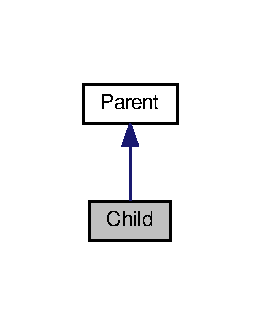
\includegraphics[width=125pt]{classChild__inherit__graph}
\end{center}
\end{figure}


Collaboration diagram for Child\+:
\nopagebreak
\begin{figure}[H]
\begin{center}
\leavevmode
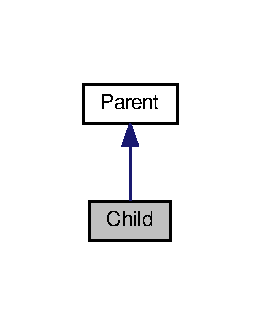
\includegraphics[width=125pt]{classChild__coll__graph}
\end{center}
\end{figure}
\subsection*{Public Member Functions}
\begin{DoxyCompactItemize}
\item 
void \hyperlink{classChild_afc9f124e971edff65cab426f1bea69df}{set\+Id} (int id)
\item 
void \hyperlink{classChild_ae869a856a652ed224a1df31e066a7b92}{display\+Id} ()
\end{DoxyCompactItemize}
\subsection*{Additional Inherited Members}


\subsection{Member Function Documentation}
\index{Child@{Child}!display\+Id@{display\+Id}}
\index{display\+Id@{display\+Id}!Child@{Child}}
\subsubsection[{\texorpdfstring{display\+Id()}{displayId()}}]{\setlength{\rightskip}{0pt plus 5cm}void Child\+::display\+Id (
\begin{DoxyParamCaption}
{}
\end{DoxyParamCaption}
)\hspace{0.3cm}{\ttfamily [inline]}}\hypertarget{classChild_ae869a856a652ed224a1df31e066a7b92}{}\label{classChild_ae869a856a652ed224a1df31e066a7b92}

\begin{DoxyCode}
32     \{
33         cout << \textcolor{stringliteral}{"id\_protected is: "} << \hyperlink{classParent_ae4415e6e7d3c3e06433ae19e1858fd45}{id\_protected} << endl;
34     \}
\end{DoxyCode}
\index{Child@{Child}!set\+Id@{set\+Id}}
\index{set\+Id@{set\+Id}!Child@{Child}}
\subsubsection[{\texorpdfstring{set\+Id(int id)}{setId(int id)}}]{\setlength{\rightskip}{0pt plus 5cm}void Child\+::set\+Id (
\begin{DoxyParamCaption}
\item[{int}]{id}
\end{DoxyParamCaption}
)\hspace{0.3cm}{\ttfamily [inline]}}\hypertarget{classChild_afc9f124e971edff65cab426f1bea69df}{}\label{classChild_afc9f124e971edff65cab426f1bea69df}

\begin{DoxyCode}
22     \{
23         
24         \textcolor{comment}{// Child class is able to access the inherited }
25         \textcolor{comment}{// protected data members of base class}
26         
27         \hyperlink{classParent_ae4415e6e7d3c3e06433ae19e1858fd45}{id\_protected} = id;
28         
29     \}
\end{DoxyCode}


The documentation for this class was generated from the following file\+:\begin{DoxyCompactItemize}
\item 
\hyperlink{AccessModifiers_8cpp}{Access\+Modifiers.\+cpp}\end{DoxyCompactItemize}

\hypertarget{classParent}{}\section{Parent Class Reference}
\label{classParent}\index{Parent@{Parent}}


Inheritance diagram for Parent\+:
\nopagebreak
\begin{figure}[H]
\begin{center}
\leavevmode
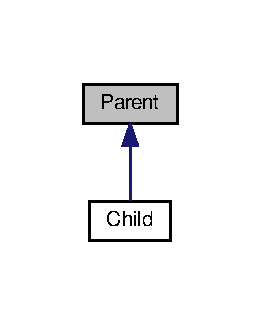
\includegraphics[width=125pt]{classParent__inherit__graph}
\end{center}
\end{figure}
\subsection*{Protected Attributes}
\begin{DoxyCompactItemize}
\item 
int \hyperlink{classParent_ae4415e6e7d3c3e06433ae19e1858fd45}{id\+\_\+protected}
\end{DoxyCompactItemize}


\subsection{Member Data Documentation}
\index{Parent@{Parent}!id\+\_\+protected@{id\+\_\+protected}}
\index{id\+\_\+protected@{id\+\_\+protected}!Parent@{Parent}}
\subsubsection[{\texorpdfstring{id\+\_\+protected}{id_protected}}]{\setlength{\rightskip}{0pt plus 5cm}int Parent\+::id\+\_\+protected\hspace{0.3cm}{\ttfamily [protected]}}\hypertarget{classParent_ae4415e6e7d3c3e06433ae19e1858fd45}{}\label{classParent_ae4415e6e7d3c3e06433ae19e1858fd45}


The documentation for this class was generated from the following file\+:\begin{DoxyCompactItemize}
\item 
\hyperlink{AccessModifiers_8cpp}{Access\+Modifiers.\+cpp}\end{DoxyCompactItemize}

\chapter{File Documentation}
\hypertarget{AccessModifiers_8cpp}{}\section{Access\+Modifiers.\+cpp File Reference}
\label{AccessModifiers_8cpp}\index{Access\+Modifiers.\+cpp@{Access\+Modifiers.\+cpp}}
{\ttfamily \#include $<$bits/stdc++.\+h$>$}\\*
Include dependency graph for Access\+Modifiers.\+cpp\+:
\nopagebreak
\begin{figure}[H]
\begin{center}
\leavevmode
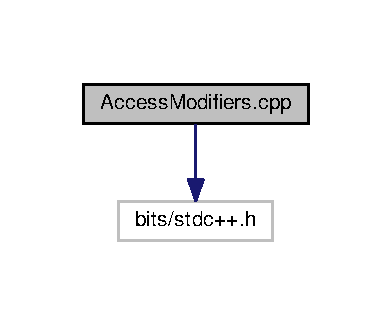
\includegraphics[width=188pt]{AccessModifiers_8cpp__incl}
\end{center}
\end{figure}
\subsection*{Classes}
\begin{DoxyCompactItemize}
\item 
class \hyperlink{classParent}{Parent}
\item 
class \hyperlink{classChild}{Child}
\end{DoxyCompactItemize}
\subsection*{Functions}
\begin{DoxyCompactItemize}
\item 
int \hyperlink{AccessModifiers_8cpp_ae66f6b31b5ad750f1fe042a706a4e3d4}{main} ()
\end{DoxyCompactItemize}


\subsection{Function Documentation}
\index{Access\+Modifiers.\+cpp@{Access\+Modifiers.\+cpp}!main@{main}}
\index{main@{main}!Access\+Modifiers.\+cpp@{Access\+Modifiers.\+cpp}}
\subsubsection[{\texorpdfstring{main()}{main()}}]{\setlength{\rightskip}{0pt plus 5cm}int main (
\begin{DoxyParamCaption}
{}
\end{DoxyParamCaption}
)}\hypertarget{AccessModifiers_8cpp_ae66f6b31b5ad750f1fe042a706a4e3d4}{}\label{AccessModifiers_8cpp_ae66f6b31b5ad750f1fe042a706a4e3d4}

\begin{DoxyCode}
38            \{
39     
40     \hyperlink{classChild}{Child} obj1;
41     
42     \textcolor{comment}{// member function of derived class can}
43     \textcolor{comment}{// access the protected data members of base class}
44     
45     obj1.\hyperlink{classChild_afc9f124e971edff65cab426f1bea69df}{setId}(81);
46     obj1.\hyperlink{classChild_ae869a856a652ed224a1df31e066a7b92}{displayId}();
47     \textcolor{keywordflow}{return} 0;
48 \}\end{DoxyCode}


Here is the call graph for this function\+:
\nopagebreak
\begin{figure}[H]
\begin{center}
\leavevmode
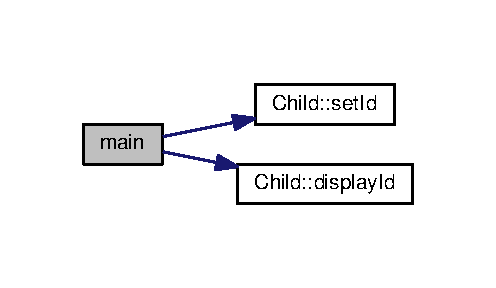
\includegraphics[width=238pt]{AccessModifiers_8cpp_ae66f6b31b5ad750f1fe042a706a4e3d4_cgraph}
\end{center}
\end{figure}



%--- End generated contents ---

% Index
\backmatter
\newpage
\phantomsection
\clearemptydoublepage
\addcontentsline{toc}{chapter}{Index}
\printindex

\end{document}
